\begin{surferIntroPage}{Superficies Record}{record_chmutovoktic}{Superficies Récord}
    Una superficie es llamada \emph{no singular} o \emph{lisa} si, como la esfera o el toro,
    no tiene \emph{singularidades}, es decir no tienen puntas o aristas. Casi cualquier superficie que elijamos al azar será no singular.
 \begin{center}
      \vspace{-0.2cm}
      \begin{tabular}{@{}c@{}c@{}c@{\quad}c@{}c@{}c@{}c@{}}
        \begin{tabular}{@{}c@{}}
          Lisa:
        \end{tabular}
        &
        \begin{tabular}{@{}c@{}}
          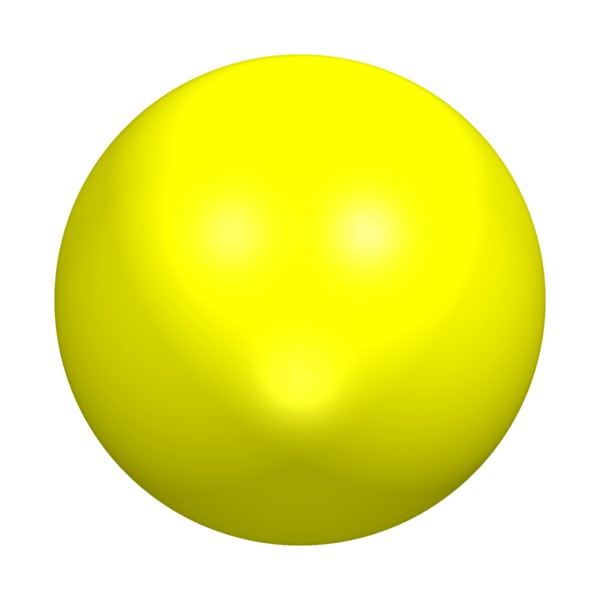
\includegraphics[width=1.1cm]{../../common/images/kugel}
        \end{tabular}
        &
        \begin{tabular}{@{}c@{}}
          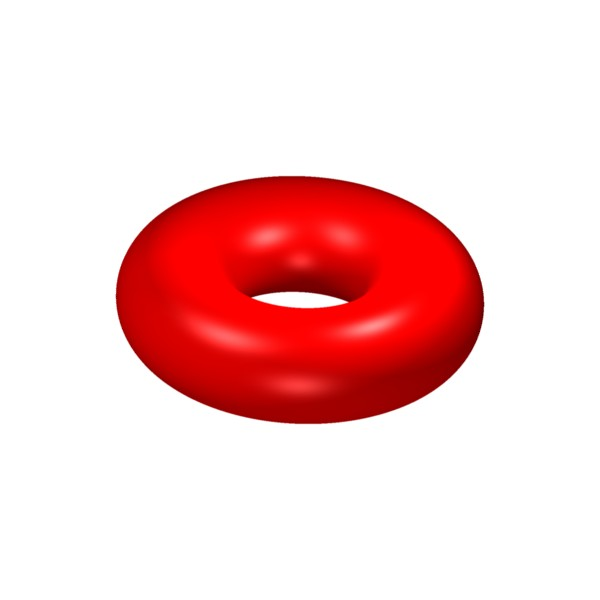
\includegraphics[width=1.1cm]{../../common/images/torus}
        \end{tabular}
        &
        \begin{tabular}{@{}c@{}}
          Muchas\\
          singularidades:
        \end{tabular}
        &
        \begin{tabular}{c@{}@{}}
          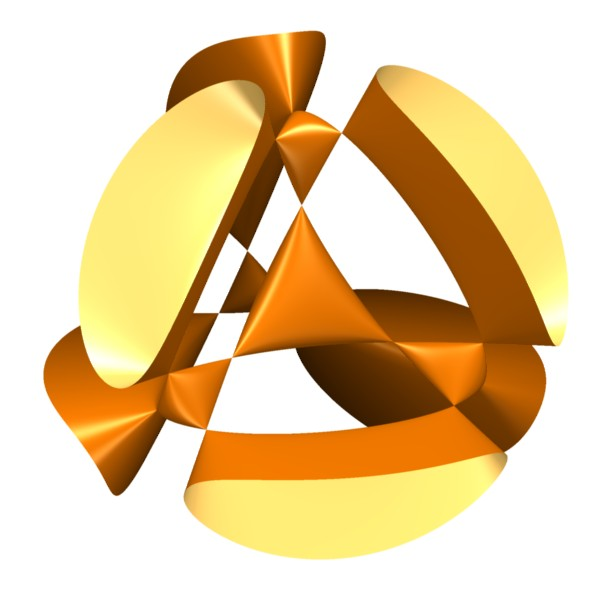
\includegraphics[width=1.1cm]{../../common/images/kummer}
        \end{tabular}
        &
        \begin{tabular}{c@{}@{}}
          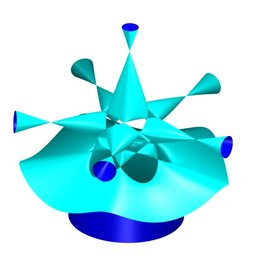
\includegraphics[width=1.1cm]{../../common/images/togliatti}
        \end{tabular}
        &
        \begin{tabular}{c@{}@{}}
          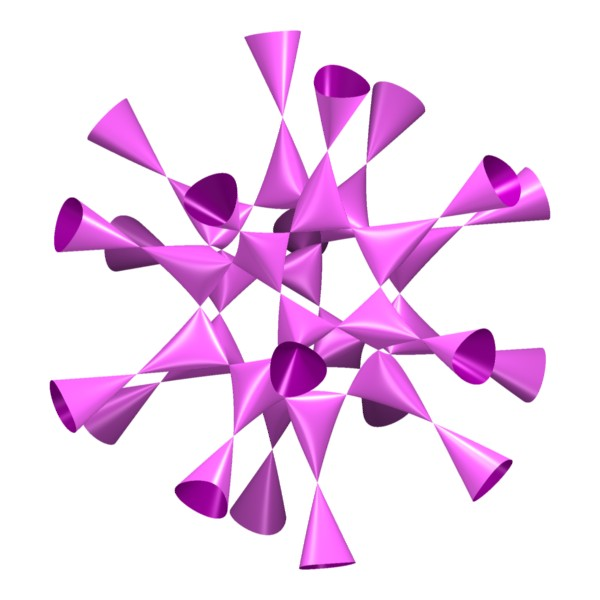
\includegraphics[width=1.1cm]{../../common/images/barth_sextic}
        \end{tabular}
      \end{tabular}
    \end{center}
    \vspace{-0.2cm}
    Por lo tanto, una superficie que tenga singularidades es muy especial.
    Ahora bien, es natural pensar cuántas singularidades puede llegar a tener una
    superficie algebraica, según el grado $d$ del polinomio que la define.  
    La determinación de este número, que denotamos $\mu(d)$, es muy difícil de calcular.

    En el siglo XIX, se conocieron los valores de $\mu(d)$ para los casos $d=1,2,3,4$. Pero para $d=5$ 
    y $d=6$ no fueron descubiertos sino hasta los años 1980 y 1996, respectivamente.
    Desde entonces, se han obtenido algunos resultados parciales para $d\ge 7$, pero la
    respuesta definitiva para el caso general es aún incierta.
  
    Algunos resultados conocidos:
    
   \begin{center}
      \begin{tabular}{r|cccccccc|c}
        $d$ & $1$ & $2$ & $3$ & $4$ & $5$ & $6$ & $7$ & $8$ & $d$\\
        \hline
        \hline
        \rule{0pt}{1.2em}$\mu(d)\ge$ & $0$ & $1$ & $4$ & $16$ & $31$ & $65$ &
        $99$ & $168$ & 
        $\approx \frac{5}{12}d^3$\\[0.3em]
        \hline
        \rule{0pt}{1.2em}$\mu(d)\le$ & $0$ & $1$ & $4$ & $16$ & $31$ & $65$ &
        $104$ & $174$ & $\approx \frac{4}{9}d^3$
      \end{tabular}
    \end{center}
  \end{surferIntroPage}
  